\chapter{Conclusion} % top level followed by section, subsection

\section{Future Work}

This paper discusses various issues regarding the development of 
The HCMP Player. The HCMP Player itself is part of a larger HCMP project 
that facilitates music representation, preparation, and performance.
There are some components that can be built upon the HCMP Player and some 
what can be directly integrated with the HCMP Player. Two
features can be added to further extend the HCMP Player's functionality. 

\subsection{Integrate with Score Display}
HCMP has a score display component which is also developed with Serpent.
Figure 7.1 is a screenshot of the score display component. The score 
display component can be used to notate a music score and turn
pages. Since the HCMP Player described here and the score display 
are really just two different specializations of the Player class,
both can be controlled by a Conductor object which will keep them synchronized.

Although the score display component illustrated here was used in earlier 
HCMP prototypes, a newer display component has been developed by Zeyu.

%The original score following component has a built-in player function,
%and it can easily be replaced by the HCMP Player. With a set of predefined API 
%of HCMP Player, score following components can be easily extended to coperate 
%with the HCMP Player. The HCMP Player will synchronize with score following 
%components by constantly receiving commands through the network. 

\begin{figure}[H]
\center{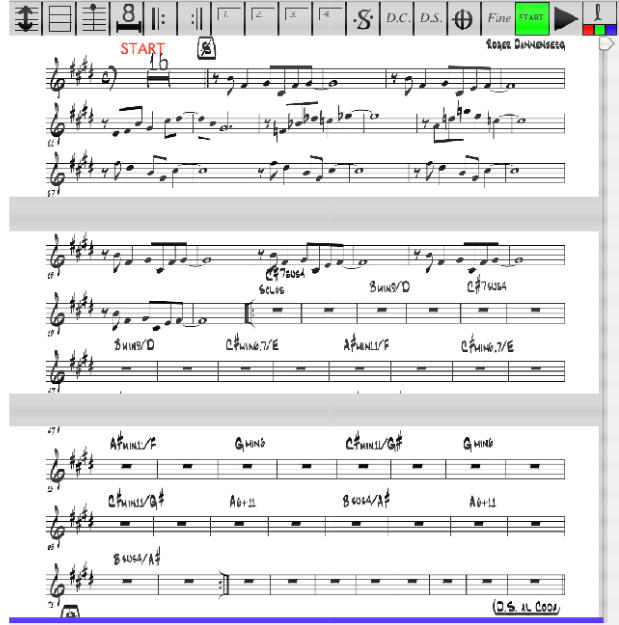
\includegraphics[width=0.5\linewidth]{8/1.png}}
\caption{HCMP Score Display Component \cite{Dawen:ISMIR2011}}
\end{figure}

\subsection{Integrate with Midi Database}
Another interesting application relates to MIDI Database \cite{Dawen:ISMIR2011} 
based on Dawen Liang's previous work. The basic idea of a MIDI Database 
is to create a tool by which a user is able to quickly record, organize
and retrieve audio information from various sources. The HCMP could be  
integrated with a MIDI Database, so that users can easily play MIDI 
segments resulting from  Database queries.

\section{Conclusion}
From the HCMP project's perspective, the HCMP Player is a building block for a 
larger project. It can also cooperate with other components to create other
applications. From a developer's perspective, the HCMP Player provides an API
which can be extended and tailored to fit into a more sophisticated project.
The HCMP Player can be split into 3 parts:  
GUI, player engine and network. The design and usage of each part 
is explained in detail in the previous chapters. I also briefly describe 
the implementation of each part. Some pseudocode segments are provided to 
illustrate logic. A complete list of the HCMP Player features is provided 
and the project has been evaluated according to a set of criteria for success. 

As an open-source MIDI player with facilities for network control, 
synchronization, visualization of sequences, and a graphical user interface,
I hope that the HCMP Player will find many application's as a component of 
interactive music systems.
